\documentclass{beamer}

\mode<presentation>{\usetheme{Madrid}}
\usepackage{graphicx}
\usepackage{booktabs}
\usepackage{lmodern}
\usepackage{epstopdf}
\usepackage[ngerman]{babel}
\usepackage[T1]{fontenc}
\usepackage[latin9]{inputenc}
\usepackage{enumerate}
\usepackage{geometry}
\usepackage{tikz}

\setbeamertemplate{items}[square]

\newtheorem{proposition}[theorem]{Satz}
\newtheorem{conjecture}[theorem]{Vermutung}
\newtheorem{remark}[theorem]{Bemerkung}
\newcommand{\DF}[1]{{\bf #1\/}}

%BESONDERE SCHRIFTARTEN:

\newcommand{\cG}{{\cal G}}
\newcommand{\cE}{{\cal EG}}

%GRAPHENPARAMETER

\newcommand{\De}{\Delta}
\newcommand{\om}{\omega}
\newcommand{\al}{\alpha}
\newcommand{\cn}{\chi}

%DATUM

\def\datum{26. September 2014}

% MENGEN

\newcommand{\N}{{\mathbb{N}}}
\newcommand{\Z}{{\mathbb{Z}}}
\newcommand{\R}{{\mathbb{R}}}
\newcommand{\C}{{\mathbb{C}}}
\newcommand{\Rnn}{{\mathbb{R}^{n\times n}}}

% SONSTIGES

\newcommand{\tr}{\operatorname{trace}}
\newcommand{\set}[2]{\{#1 \;|\; #2 \}}
\newcommand{\ems}{\varnothing}
\newcommand{\sm}{\setminus}
\newcommand{\la}{\langle}
\newcommand{\ra}{\rangle}


\title[Chrom. Zahl und Spektrum von Graphen]{Chromatische Zahl und Spektrum von Graphen}
\author[Stefan Heyder]{Stefan Heyder \\ Betreuer: Prof. Dr. Stiebitz}


\institute{TU Ilmenau}
\date{30. September 2014}

\begin{document}
\begin{frame}[<+->]
  \titlepage
\end{frame}

\begin{frame}[<+->]
  \frametitle{Inhalt} 
  \tableofcontents 
\end{frame}

\begin{frame}[<+->]
  \setbeamercovered{dynamic}
  \frametitle{Ein F"arbungsproblem}
  Es sei $\cE(n)$ die Klasse aller Graphen, welche die kantendisjunkte Vereinigung von $n$ vollst"andigen Graphen der Ordnung $n$ sind.
  %% TODO: Bilder
\end{frame}

\section{Die Erd\H os-Faber-Lov\'asz Vermutung}

\begin{frame}[<+->]
  \setbeamercovered{dynamic}
  \frametitle{Die Erd\H{o}s-Faber-Lov\'asz Vermutung}
  \begin{conjecture}[Erd\H{o}s-Faber-Lov\'asz(1972)]
    Sei $G\in\cE(n)$. Dann gilt $\chi(G) \leq n$.
  \end{conjecture}
  \pause
  Ein Hypergraph $H$ hei{\ss}t \DF{linear}, falls $|e\cap e'| \leq 1$ f"ur alle $e,e'\in E(H)$.
  \pause
  \begin{conjecture}
    Sei $H$ ein linearer Hypergraph. Dann gilt $\chi'(H) \leq |H|$.
  \end{conjecture}
\end{frame}

\begin{frame}[<+->]
  \setbeamercovered{dynamic}
  \frametitle{Die Erd\H{o}s-Faber-Lov\'asz Vermutung}
  \begin{theorem}[Chung \& Lawler]
    F"ur jeden Graphen $G\in \cE(n)$ gilt $\chi(G) \leq \frac{3n}{2} -2$.
  \end{theorem}
  \begin{theorem}[Kahn]
    F"ur jeden linearen Hypergraphen $H$ ist $\chi'(H) \leq |H| + o(|H|)$.
  \end{theorem}
\end{frame}

\begin{frame}[<+->]
  \setbeamercovered{dynamic}
  \frametitle{Krauszzerlegungen}
    Eine Menge von Untergraphen $\mathcal{K}$ von $G$ hei{\ss}t \DF{Krauszzerlegung} von $G$, falls gilt:
    \pause
    \begin{enumerate}[<+->]
      \item Alle $K\in \mathcal{K}$ sind vollst"andige Graphen der Ordnung $|K| \geq 2$.
      \item Sind $K,K'\in \mathcal{K}$ verschieden, so gilt $|K\cap K'| \leq 1$.
      \item $\bigcup\limits_{K\in \mathcal{K}} K = G$.
    \end{enumerate}
  %% TODO: Bilder
\end{frame}

\begin{frame}[<+->]
  \setbeamercovered{dynamic}
  \frametitle{Krauszzerlegungen}
  \begin{itemize}[<+->]
    \item $d_{\mathcal{K}}(v) = | \set{K\in \mathcal{K}}{v\in K}| $, der \DF{Grad} von $v$ in $\mathcal{K}$.
    \item $\delta(\mathcal{K})$, der \DF{Minimalgrad} .
    \item $\kappa_{d}(G)$, die kleinste Zahl $p$, sodass $G$ eine Krauszzerlegung $\mathcal{K}$ mit $|\mathcal{K}| = p$ besitzt ($\kappa_{d}(G) = \infty$, falls kein solches $p$ existiert).
  \end{itemize}
  %% TODO: Bilder
\end{frame}

\begin{frame}[<+->]
  \setbeamercovered{dynamic}
  \frametitle{Krauszzerlegungen und die Erd\H os-Faber-Lov\'asz Vermutung}
  \begin{theorem}
    Die folgenden Aussagen sind "aquivalent:
    \begin{enumerate}[<+->]
      \item F"ur alle Graphen $G\in \cE(n)$ gilt $\chi(G) \leq n$.
      \item F"ur alle Graphen $G$ gilt $\chi(G) \leq \kappa_{2}(G)$.
      \item F"ur alle linearen Hypergraphen $H$ gilt $\chi'(H) \leq |H|$.
    \end{enumerate}
  \end{theorem}
\end{frame}

\begin{frame}
  \setbeamercovered{dynamic}
  \frametitle{Krauszzerlegungen und die Erd\H os-Faber-Lov\'asz Vermutung}
\begin{figure}[h]
  \centering
  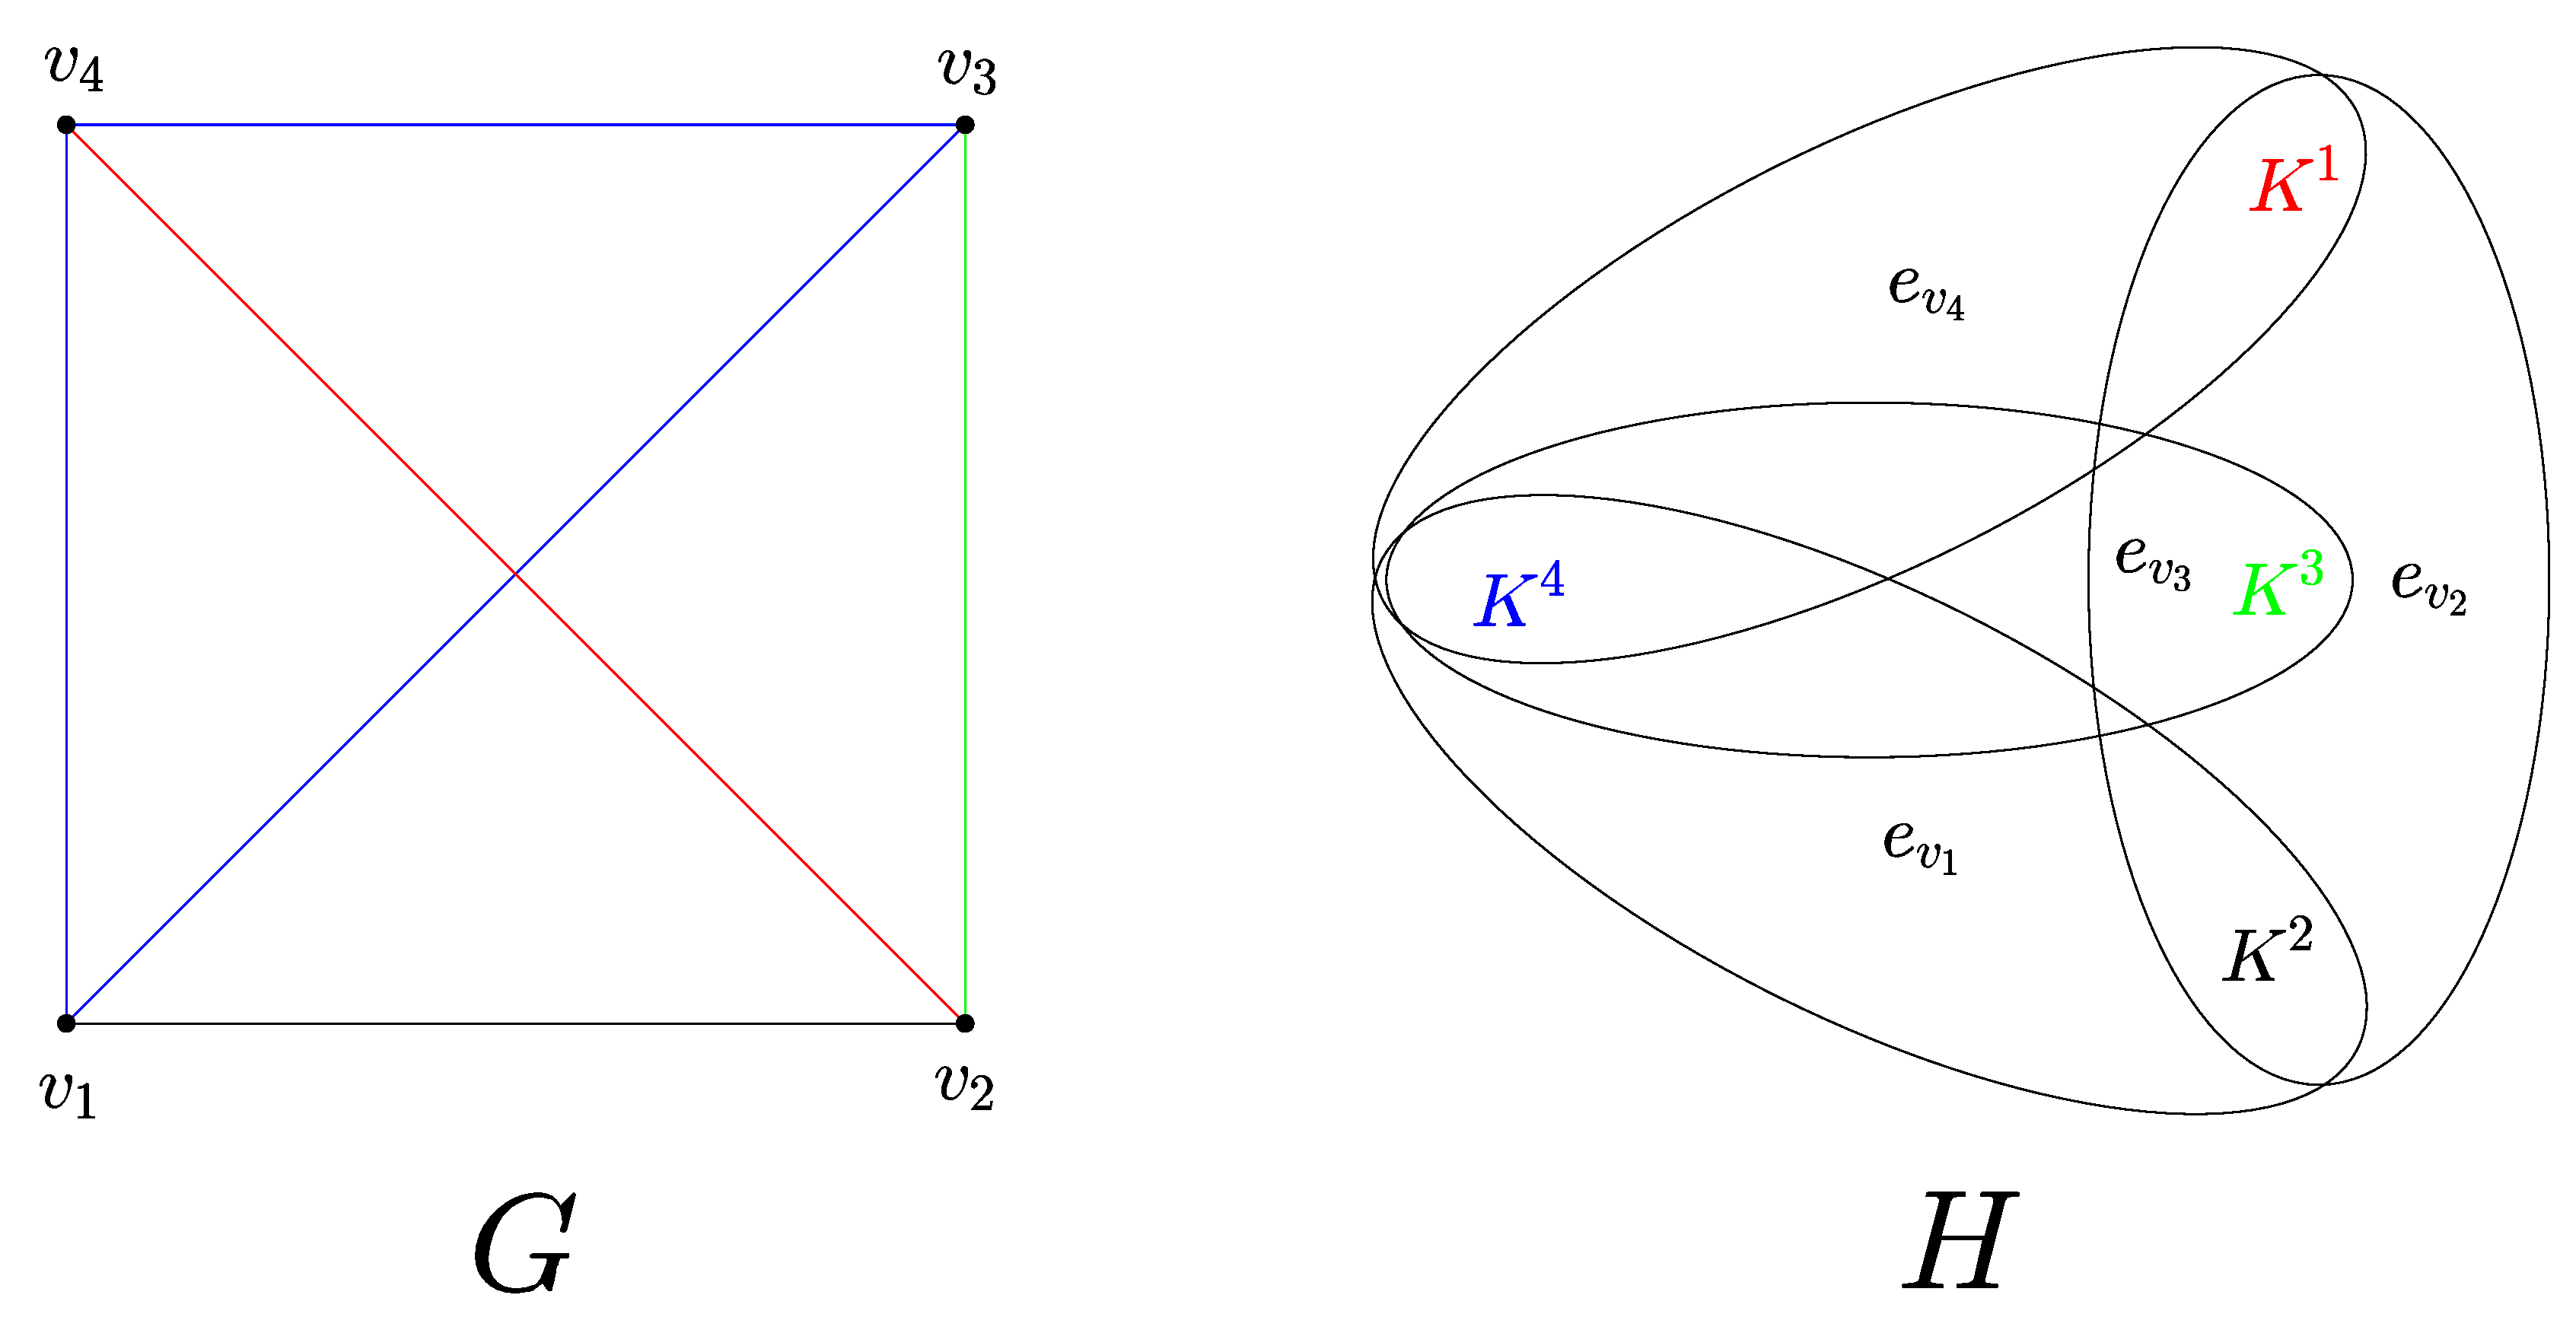
\includegraphics[width=\textwidth]{images/k4krausztohypergraph}
\end{figure}
\end{frame}
\begin{frame}
  \setbeamercovered{dynamic}
  \frametitle{Krauszzerlegungen und die Erd\H os-Faber-Lov\'asz Vermutung}
  \begin{figure}[h]
    \centering
    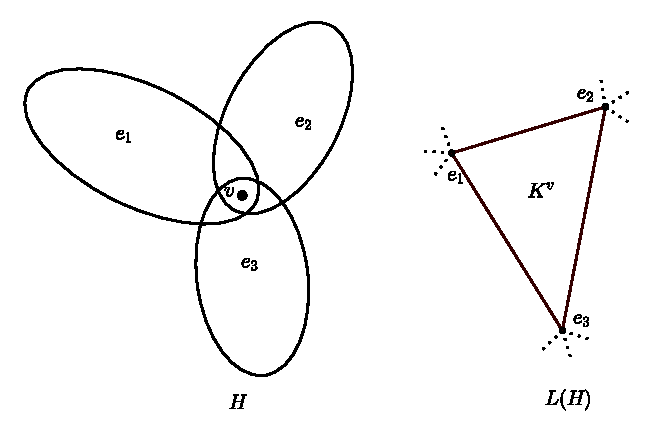
\includegraphics[width=\textwidth]{images/KvLinegraph.eps}
  \end{figure}
\end{frame}
\section{Eigenwerte von Graphen}
\begin{frame}[<+->]
  \setbeamercovered{dynamic}
  \frametitle{Eigenwerte von Graphen}
  Es sei $A(G)$ die \DF{Adjazenzmatrix} von $G$ mit 
  $$A(G)_{ij} = \begin{cases}
    1 & \text{, falls } v_iv_j \in E(G) \\
    0 & \text{, sonst.}
  \end{cases}$$
  \pause
  Die \DF{Eigenwerte} von $G$ sind dann die Eigenwerte von $A(G)$. 
  \pause
  Wir bezeichnen mit $\lambda_{i}(G)$ den $i$-gr"o{\ss}ten Eigenwert von $G$. Also gilt 
  $$\lambda_{max}(G) = \lambda_{1}(G) \geq \lambda_{2}(G) \geq \dots \geq \lambda_{n}(G) = \lambda_{min}(G).$$
\end{frame}


\begin{frame}
  \setbeamercovered{dynamic}
  \frametitle{Chromatische Zahl und Eigenwerte}
  \begin{theorem}[Wilf]
    Ist $G$ ein zusammenh"angender Graph, so gilt $\chi(G) \leq \lambda_{1}(G) +1$.
  \end{theorem}
  \begin{theorem}[Hoffman]
    Ist $G$ ein Graph, so gilt $\chi(G) \geq 1- \frac{\lambda_{max}(G)}{\lambda_{min}(G)}$.
  \end{theorem}
\end{frame}
\begin{frame}[<+->]
  \setbeamercovered{dynamic}
  \frametitle{Krauszzerlegungen und Eigenwerte}
  \begin{theorem}
    Sei $\mathcal{K} = \{K^{1}, K^{2}, \dots , K^{p} \}$ eine Krauszzerlegung von $G$. Wir setzen $d_i = d_{\mathcal{K}}(v_i)$, wobei wir die Nummerierung der Ecken so w"ahlen, dass $d_1 \geq d_2 \geq \dots \geq d_n$ gilt.
    Dann gelten folgende Aussagen:
    \begin{enumerate}
      \item $\lambda_{i}(G) \geq -d_{n-i+1}$ f"ur alle $1 \leq i \leq n$. 
      \item $\lambda_{p+1}(G) \leq -d_n$, falls $p< n$.
    \end{enumerate}
  \end{theorem}
\end{frame}
\begin{frame}[<+->]
  \setbeamercovered{dynamic}
  \frametitle{Krauszzerlegungen und Eigenwerte}

  Es seien $A= A(G)$, $D= \operatorname{diag}(d_1,d_2,\dots,d_n)$ und $B\in\R^{n\times p}$ die Inzidenzmatrix von $\mathcal{K}$. Dann gilt
  $$ B_{ij} = \begin{cases}
    1 & \text{ falls } v_i\in K^{j} \\
    0 & \text{ sonst.} 
  \end{cases} $$
  \pause
  Sei $M=BB^{T}$. Dann ist $M$ positiv semidefinit und $M=A+D$, wie sich leicht zeigen l"asst. \pause Also folgt 
  $$\lambda_{i}(A) \geq \lambda_{i}(-D) = -\lambda_{n-i+1}(D) = -d_{n-i+1}$$
  \pause
  Ist $p < n$, so ist $\operatorname{rang}(M) = \operatorname{rang} (B) \leq p < n$, insbesondere ist $\lambda_{p+1}(M) = 0$. 
  \pause
  Somit gilt
  $$\lambda_{p+1}(A) + d_n \leq \lambda_{p+1}(M) = 0. $$
\end{frame}

\begin{frame}[<+->]
  \setbeamercovered{dynamic}
  \frametitle{Eigenwerte von Graphen}
  \begin{itemize}[<+->]
    \item F"ur $d\in \N$ sei $\xi_{d}(G) = | \set{i \in \N}{\lambda_{i}(G) > -d}|$.
    \item Es ist leicht zu zeigen, dass $\xi_{d}(G) \leq \kappa_{d}(G)$ gilt.
  \end{itemize}
  \begin{conjecture}
    F"ur alle Graphen $G$ gilt $\chi(G) \leq \xi_{2}(G)$.
  \end{conjecture}
\end{frame}

\begin{frame}[<+->]
  \setbeamercovered{dynamic}
  \frametitle{Graphen mit $\chi \leq \xi_{2}$}
  \pause
  Vermutung gilt f"ur 
  \pause
  \begin{itemize}
    \item Graphen $G$ mit $\chi(G) \leq 3$.
    \item Kneser Graphen.
    \item Planare Graphen.
    \item Perfekte Graphen.
    \item Kantengraphen.
  \end{itemize}
  \pause
\end{frame}
 \begin{frame}
   \setbeamercovered{dynamic}
   \frametitle{Graphen mit $\chi \leq \xi_{2}$}
   \begin{theorem}
     Sei $G$ ein Graph. Dann gilt $\chi(G) \leq \xi_{2}(G) \text{ oder } \chi(\overline G) \leq \xi_{2}(\overline G)$.
   \end{theorem}
 \end{frame}
\end{document}
